% Conceptual Framework — Agyemang-style relational abstraction.
% Three actors (Commuters, Workplaces, Transport network) interact through
% a central two-stage ML-ABM framework. Outputs flow to welfare assessment.
% Policy question motivates the whole figure at top.
%
% Compile: pdflatex figure_conceptual.tex

\documentclass[border=10pt]{standalone}

\usepackage[T1]{fontenc}
\usepackage{lmodern}
\usepackage{amsmath, amssymb}
\usepackage{tikz}
\usepackage{xcolor}

\usetikzlibrary{
  positioning, arrows.meta, shapes.geometric, shapes.symbols,
  shapes.misc, calc, fit, backgrounds, decorations.pathmorphing,
}

% ── Colour palette (soft, conceptual) ──────────────────────────────────
\definecolor{cActorBg}     {HTML}{E0EBF5}
\definecolor{cActorBorder} {HTML}{3B6FB6}
\definecolor{cFrameBg}     {HTML}{FAE5DD}
\definecolor{cFrameBorder} {HTML}{C44E52}
\definecolor{cStageBg}     {HTML}{FFF7E6}
\definecolor{cStageBorder} {HTML}{B8732E}
\definecolor{cOutBg}       {HTML}{D6EBE8}
\definecolor{cOutBorder}   {HTML}{0F766E}
\definecolor{cQuestion}    {HTML}{8172B2}
\definecolor{cText}        {HTML}{1F2937}
\definecolor{cMuted}       {HTML}{6B7280}
\definecolor{cFlow}        {HTML}{E07A5F}

\begin{document}

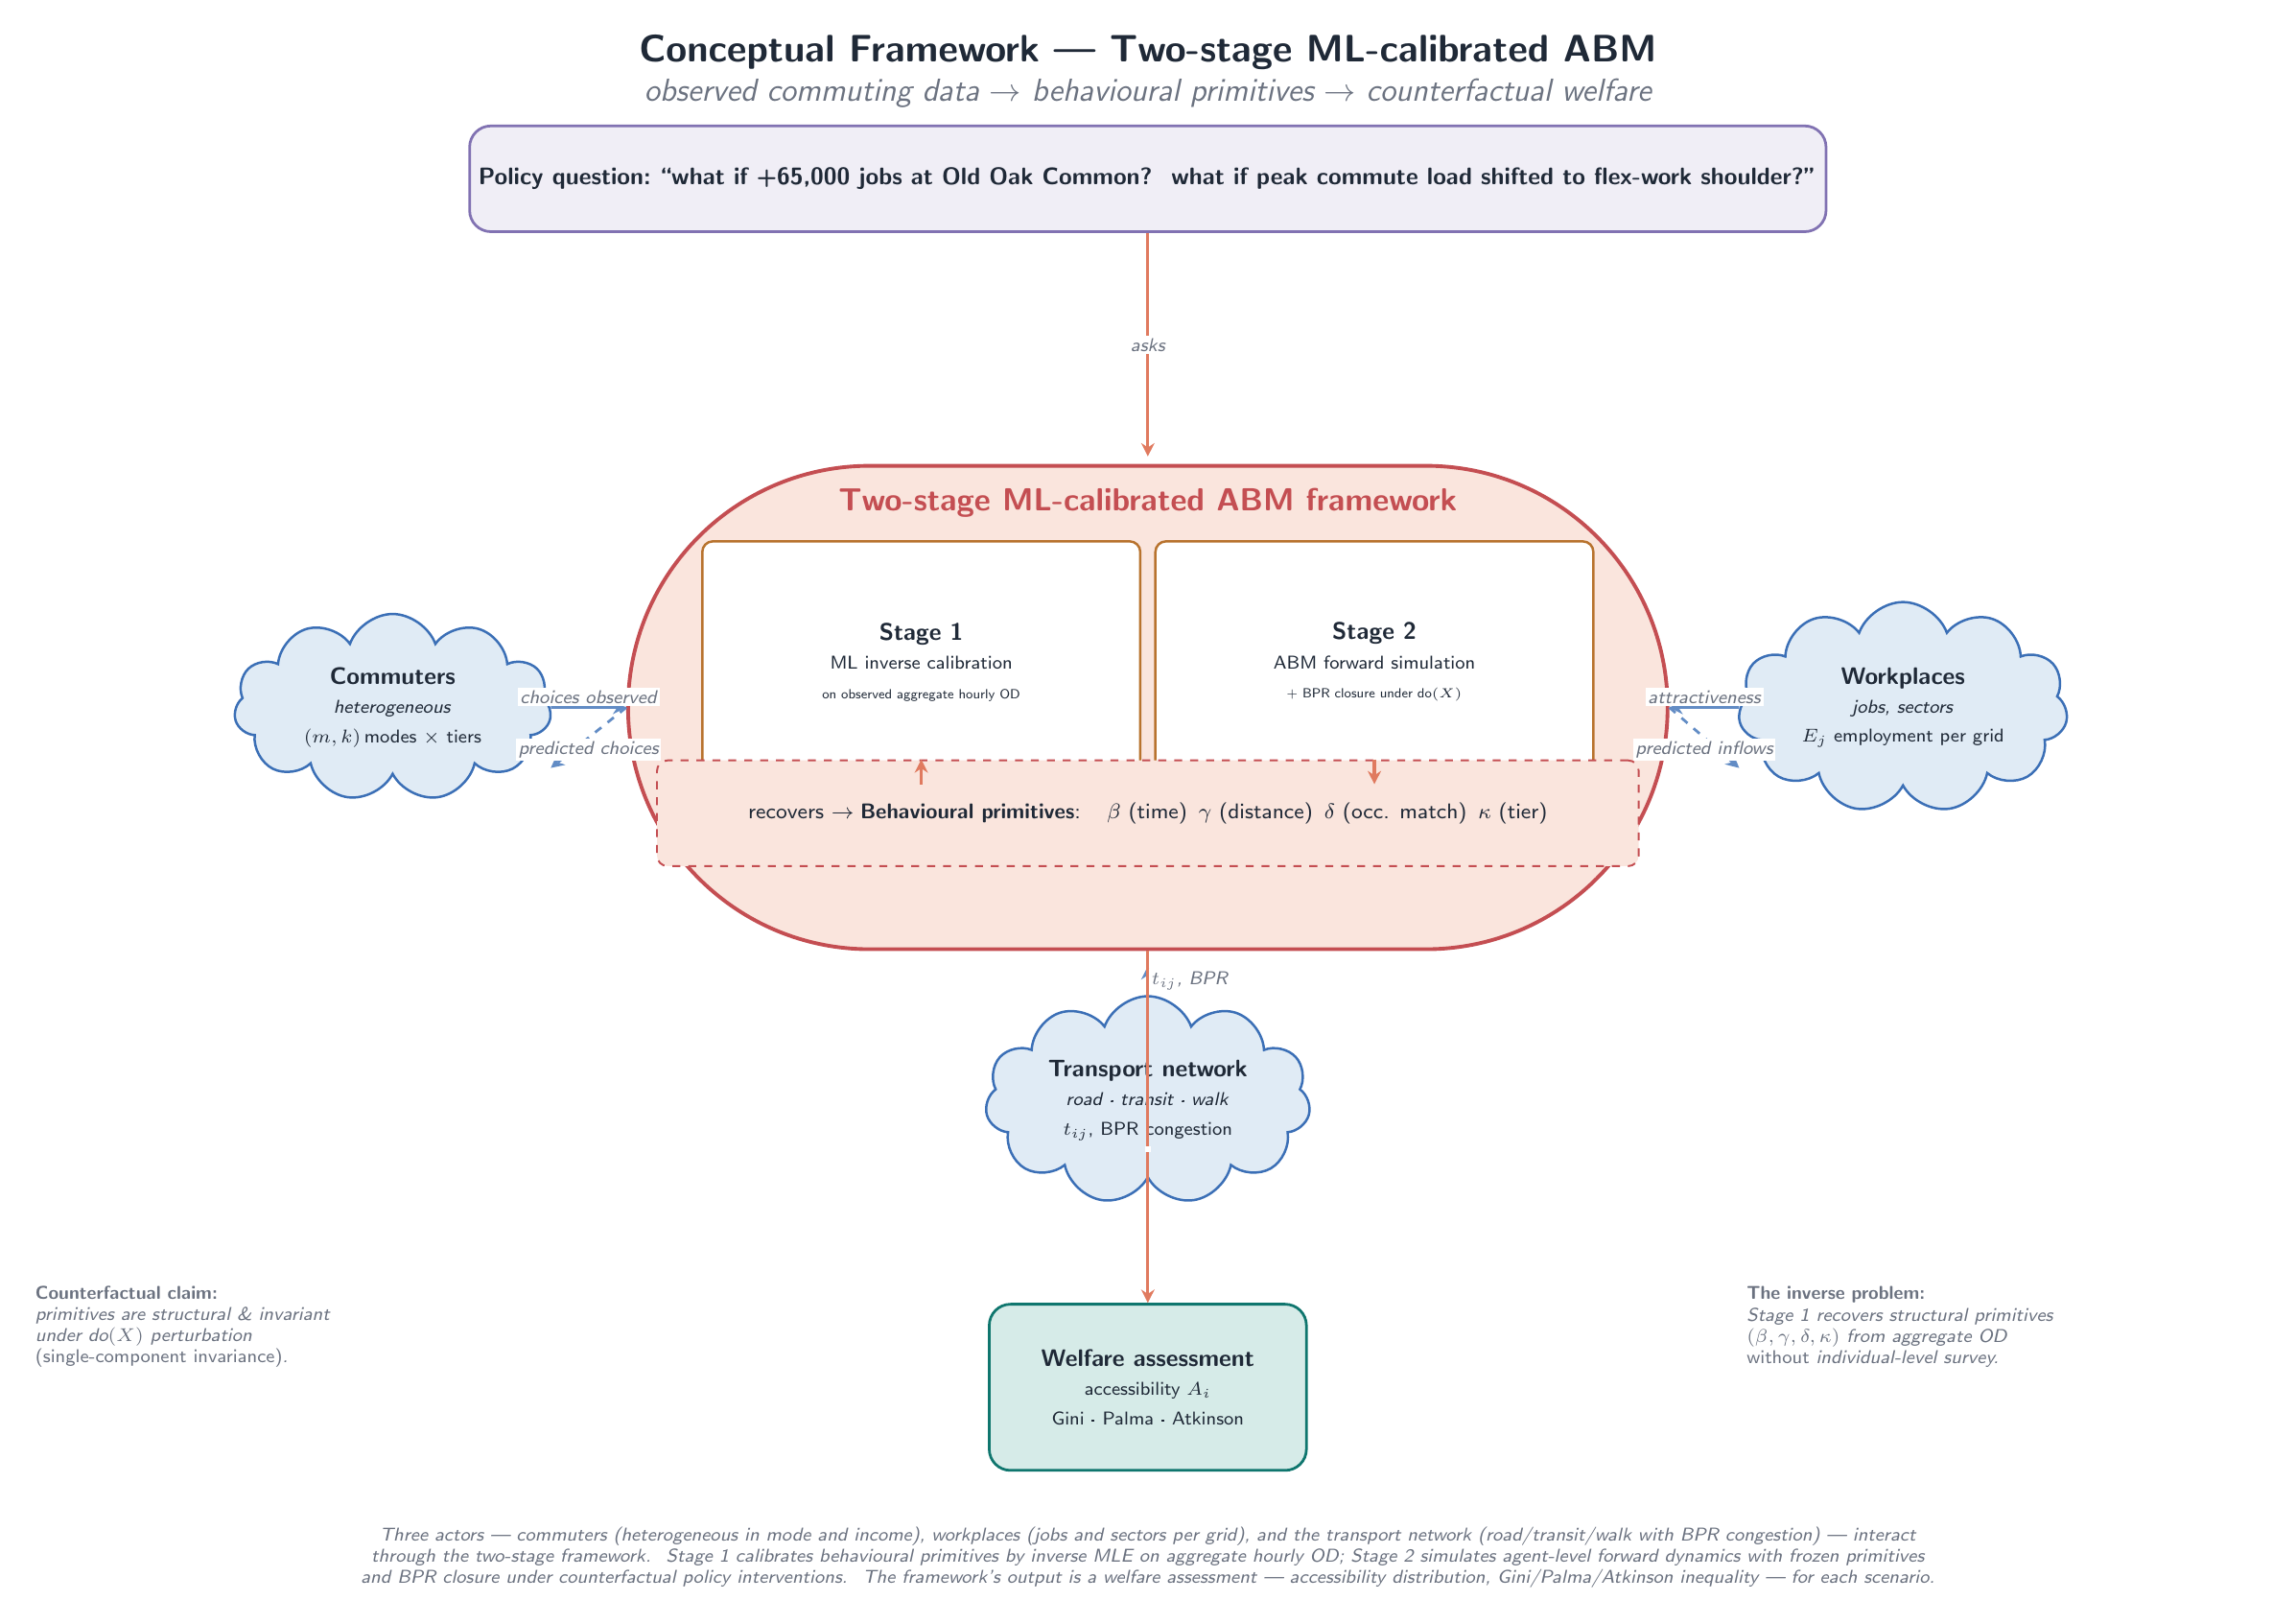
\begin{tikzpicture}[
  font=\sffamily,
  thick,
  >={Stealth[length=5pt, width=5pt]},
  every node/.style={align=center, text=cText},
  %
  actorcloud/.style={
    cloud, cloud puffs=11, cloud puff arc=140,
    draw=cActorBorder, fill=cActorBg, line width=0.9pt,
    minimum width=42mm, minimum height=24mm,
    aspect=2,
    font=\sffamily\small,
  },
  actorinside/.style={font=\sffamily\scriptsize\itshape, text=cText},
  questionbubble/.style={
    rectangle, rounded corners=8pt,
    draw=cQuestion, fill=cQuestion!12, line width=1.0pt,
    minimum width=110mm, minimum height=14mm,
    font=\sffamily\bfseries\small,
  },
  framework/.style={
    rounded rectangle, draw=cFrameBorder, fill=cFrameBg,
    line width=1.4pt,
    minimum width=140mm, minimum height=64mm,
  },
  stagebox/.style={
    rectangle, rounded corners=4pt,
    draw=cStageBorder, fill=white, line width=0.9pt,
    minimum width=58mm, minimum height=32mm,
    font=\sffamily\small,
  },
  primbox/.style={
    rectangle, rounded corners=4pt,
    draw=cFrameBorder, fill=cFrameBg, line width=0.7pt, dashed,
    minimum width=130mm, minimum height=14mm,
    font=\sffamily\footnotesize,
  },
  outputbox/.style={
    rectangle, rounded corners=8pt,
    draw=cOutBorder, fill=cOutBg, line width=1.0pt,
    minimum width=42mm, minimum height=22mm,
    font=\sffamily\small,
  },
  arrFlow/.style={->, line width=1.2pt, draw=cFlow},
  arrAct/.style={->, line width=1.0pt, draw=cActorBorder!80},
  arrlbl/.style={font=\sffamily\scriptsize\itshape, text=cMuted, fill=white,
                  inner sep=1pt, midway},
]

% ════════════════════════════════════════════════════════════════════════
%   POLICY QUESTION at top
% ════════════════════════════════════════════════════════════════════════

\node[questionbubble] (policy) at (0, 70mm)
   {Policy question:\;\itshape ``what if +65{,}000 jobs at Old Oak Common?\;
    what if peak commute load shifted to flex-work shoulder?''};

% ════════════════════════════════════════════════════════════════════════
%   THREE ACTORS (clouds, in Agyemang style) on the left, top, right
% ════════════════════════════════════════════════════════════════════════

\node[actorcloud] (commuters) at (-100mm, 0)
   {\textbf{Commuters}\\
    \textit{\scriptsize heterogeneous}\\
    \scriptsize $(m, k)$\,modes $\times$ tiers};

\node[actorcloud] (workplaces) at (100mm, 0)
   {\textbf{Workplaces}\\
    \textit{\scriptsize jobs, sectors}\\
    \scriptsize $E_j$ employment per grid};

\node[actorcloud] (transport) at (0, -52mm)
   {\textbf{Transport network}\\
    \textit{\scriptsize road · transit · walk}\\
    \scriptsize $t_{ij}$, BPR congestion};

% ════════════════════════════════════════════════════════════════════════
%   CENTRAL FRAMEWORK
% ════════════════════════════════════════════════════════════════════════

\node[framework] (frame) at (0, 0)
   {};
\node[anchor=north, font=\sffamily\bfseries\large, text=cFrameBorder]
  at ($(frame.north)+(0, -2mm)$)
   {Two-stage ML-calibrated ABM framework};

% Stage 1 box (left, inside framework)
\node[stagebox] (stage1) at (-30mm, 6mm)
   {\textbf{Stage 1}\\\scriptsize ML inverse calibration\\
    \tiny on observed aggregate hourly OD};

% Stage 2 box (right, inside framework)
\node[stagebox] (stage2) at (30mm, 6mm)
   {\textbf{Stage 2}\\\scriptsize ABM forward simulation\\
    \tiny + BPR closure under do$(X)$};

% Behavioural primitives bar (bridge between Stage 1 and Stage 2)
\node[primbox] (prim) at (0, -14mm)
   {recovers $\to$\;\textbf{Behavioural primitives}: \;
    $\beta$ (time)\, $\gamma$ (distance)\, $\delta$ (occ. match)\, $\kappa$ (tier)};

% Stage 1 → primitives → Stage 2 flow
\draw[arrFlow] (stage1.south) -- ($(prim.north)+(-30mm, 0)$);
\draw[arrFlow] ($(prim.north)+(30mm, 0)$) -- (stage2.south);

% ════════════════════════════════════════════════════════════════════════
%   OUTPUT (welfare / inequality / accessibility)
% ════════════════════════════════════════════════════════════════════════

\node[outputbox] (output) at (0, -90mm)
   {\textbf{Welfare assessment}\\
    \scriptsize accessibility $A_i$\\
    \scriptsize Gini · Palma · Atkinson};

% ════════════════════════════════════════════════════════════════════════
%   RELATIONAL ARROWS — actors interact through the framework
% ════════════════════════════════════════════════════════════════════════

% policy question → framework
\draw[arrFlow] (policy.south) --
              node[arrlbl, fill=white]{asks}
              ($(frame.north)+(0, 1mm)$);

% commuters ↔ framework
\draw[arrAct] (commuters.east) --
              node[arrlbl, above]{choices observed} (frame.west);
% workplaces ↔ framework
\draw[arrAct] (workplaces.west) --
              node[arrlbl, above]{attractiveness} (frame.east);
% transport network → framework (from below)
\draw[arrAct] (transport.north) --
              node[arrlbl, right]{$t_{ij}$, BPR} ($(frame.south)+(0, -2mm)$);

% framework → output
\draw[arrFlow] (frame.south) -- ++(0, -7mm) -|
              node[arrlbl, near end, above]{}
              (output.north);

% Framework also "drives" commuters' decisions and "shapes" workplaces' use
% (visualised as reverse-direction softer arrows)
\draw[arrAct, dashed] (frame.west) --
              node[arrlbl, below]{predicted choices} ($(commuters.east)+(0, -8mm)$);
\draw[arrAct, dashed] (frame.east) --
              node[arrlbl, below]{predicted inflows} ($(workplaces.west)+(0, -8mm)$);

% ════════════════════════════════════════════════════════════════════════
%   ANNOTATIONS — the inverse problem and counterfactual claim
% ════════════════════════════════════════════════════════════════════════

% Annotation: "the inverse problem"
\node[font=\sffamily\scriptsize\itshape, text=cMuted, anchor=west, align=left,
       text width=68mm]
  at (78mm, -82mm)
   {\textbf{The inverse problem:}\\
    Stage 1 recovers structural primitives\\
    $(\beta, \gamma, \delta, \kappa)$ from aggregate OD\\
    \emph{without} individual-level survey.};

% Annotation: "counterfactual claim"
\node[font=\sffamily\scriptsize\itshape, text=cMuted, anchor=east, align=left,
       text width=68mm]
  at (-78mm, -82mm)
   {\textbf{Counterfactual claim:}\\
    primitives are structural \& invariant\\
    under do$(X)$ perturbation\\
    \emph{(single-component invariance)}.};

% ════════════════════════════════════════════════════════════════════════
%   TITLE
% ════════════════════════════════════════════════════════════════════════

\node[font=\sffamily\bfseries\Large, anchor=south]
  at ($(policy.north)+(0, 6mm)$)
   {Conceptual Framework — Two-stage ML-calibrated ABM};
\node[font=\sffamily\itshape\large, anchor=south, text=cMuted]
  at ($(policy.north)+(0, 1mm)$)
   {observed commuting data $\to$ behavioural primitives $\to$ counterfactual welfare};

% Footer
\node[font=\sffamily\scriptsize\itshape, text=cMuted, anchor=north,
       text width=240mm]
  at ($(output.south)+(0, -6mm)$)
   {Three actors — commuters (heterogeneous in mode and income), workplaces (jobs and sectors per grid), and the transport network (road/transit/walk with BPR congestion) —
    interact through the two-stage framework.\;
    Stage 1 calibrates behavioural primitives by inverse MLE on aggregate hourly OD;
    Stage 2 simulates agent-level forward dynamics with frozen primitives and BPR closure under counterfactual policy interventions.\;
    The framework's output is a welfare assessment — accessibility distribution, Gini/Palma/Atkinson inequality — for each scenario.};

\end{tikzpicture}

\end{document}
